\section{ State-of-the-Art }
To comprehend the method of transcription, it is relevant to investigate software solutions and theoretical solutions that are approximate to the presented problem of this project. In this section the acquired solutions will be presented in conjunction with the presumed relevance which is necessary to solve the problem.

\subsection{ Voice Drummer }
Voice Drummer is defined as a "Percussion instrument notation interface" \citep{VoiceDrummer}. It is a software-application developed to aid those without substantial musical knowledge to notate music. The program is limited to transcribing bass drum and snare drum, and these are differentiated between by their onomatopoeic expressions and the rhythm-pattern timing.
\\
\begin{figure}[h]
	\begin{center}
		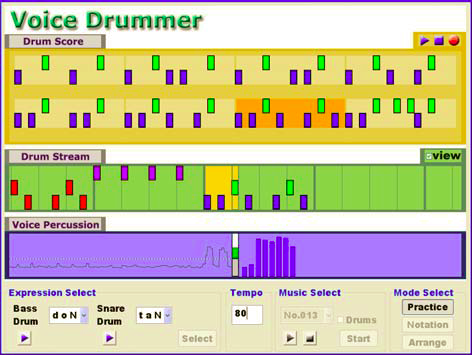
\includegraphics[height=5cm]{fig/VoiceDrummer.png}
		\caption{An example voice drummers practice adaption-mode \citep{VoiceDrummer}}
		\label{VoiceDrummer}
	\end{center}
\end{figure}
\\
Onomatopoeic refers to words that phonetically imitates, or resembles the source of the described sound e.g. classifying 'Meow' as a sound a cat would make. Thus, making it easy for a layman to understand, and use Voice Drummer by uttering \textit{don-don} to generate a Bass Drum, and \textit{ta-ta} to generate a snare drum. These are transcribed into phonemic representations through a pronunciation dictionary which will recognize and
 output the correct corresponding output in real-time.

\subsection{ Voice Band }
\begin{figure}[h]
	\begin{center}
		\includegraphics[height=5cm]{fig/voiceband.png}
		\caption{Voice Band. photo of the interface on a ipad mini}
		\label{VoiceBand}
	\end{center}
\end{figure}

Voice Band is an iPhone application by WaveMachine Labs which alters your voice into sampled instruments in real-time. It comes with a set of instruments to choose from including rhythm guitar, lead guitar, bass, sax, synthesizers, organ, drums and microphone, but there are other instruments and expansions available for purchase in the Voice Band store, e.g. other drum kits or strings. The target users are, according to WaveMachine Labs’ website and demo videos, songwriters who want an idea or arrangement down quickly; they call it a “portable musical scratch board”. However, it might also appeal and inspire anyone else interested in music, who wants to have fun. \\

For every instrument, excluding the drums and cymbals, the system detects the pitch of the voice, and changes that into an instrumental output. To avoid distortion or unwanted noise, one will get the best results by using a pair of headphones, and staying in a quiet environment, because the system is very sensitive sound. It is also recommended to use solid, pure tones with no vibrato to reach a more accurate output, and to sing with hard consonants such as ba or da, because Voice Band recognizes the start of a sound, and it is therefore easier to detect.  \\

As for the drums, they are divided into kick/snare (two-in-one), hi-hat and crash. The kick and snare drums are together, where quiet will output kick, and loud notes will output snare. However there is the possibility to adjust the sensibility on a trigger in settings, such that only kick or only snare will be outputted, not depending on the loudness of the note. This way it is possible to record kick and snare separately as well. The hi-hat system works similarly in which soft notes produces a closed hi-hat and loud notes produces an open hi-hat, Crash is for itself. For all drums, and most of the other instruments, one can adjust reverberation and volume. 
All instruments and singing will have to be recorded separately, but on the same track. After having recorded an instrument, it will play back the previous recorded sounds while recording another one. It is possible to undo the last take without having to delete everything, but if you want to edit some of the first recordings this is not possible.  You cannot go back and change or edit the whole arrangement. It converts the samples into a MP3 file, which can be sent to an e-mail. 

\subsection{ Loop Station RC-505 }
\label{loopstation}
\begin{figure}[h]
	\begin{center}
		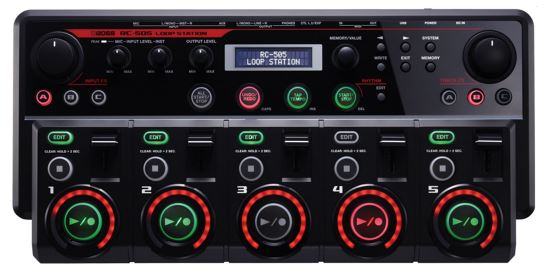
\includegraphics[height=5cm]{fig/Roland-RC-505.JPG}
		\caption{Roland Looper RC-505, picture from http://www.musicradar.com/}
		\label{Looper}
	\end{center}
\end{figure}
The Roland Loop Station is specially build for beatboxers. It enables a performing beatbox artist to record and play 5 tracks simultaneously. It can also apply sound effects to the recorded tracks, which actually makes it sound closer to a synthesizer. The Loop Station can record 99 phrases, and provides 85 on-board rhythm patterns. Moreover it can be operated with hands and with foot-switches. Additionally it can be used as a MIDI controller. It has a XLR mic input, phantom power, mono/stereo instruments input, and AUX input, which makes the Roland Looper RC-505 stands, according to Roland CONNECT, out as one of the most professional build tools for beatboxers\footnote{\url{http://www.rolandconnect.com/product_2013-04.php?p=rc-505}}.
The Loop Station is used and promoted by the Australian beatboxing-artist DUB FX.


